\chapter{Evaluierung \& Diskussion}
\label{cha:Tests und Evaluierung}

\section{.NET Klassenbibliothek und AL-Sprachkonstrukte}
\subsection{Testaufbau}
Im ersten Testaufbau werden die im Treuepunkt-Beispiel \ref{sec:Aufgabenstellung} verwendeten Varianten der Webdienst Kommunikation gemessen und auf ihr Laufzeitverhalten untersucht. In diesem Test werden beide Varianten eine große Anzahl von Http-Anfragen erstellen und an einen Webdienst übermitteln. Um die Ergebnisse vergleichbar zu halten, muss in beiden Varianten dasselbe JSON erstellt und übermittelt werden. Bei einer Messung dieser Art sind grundsätzlich immer hohe Schwankungen zu erwarten, da sowohl die momentane Netzwerklast, als auch die Verarbeitungszeit des Webdienstes mitgemessen wird. Um diese Seiteneffekte zu minimieren, beziehungsweise sie konstant zu halten, wird in diesem Test an einen eigens erstellten Webdienst übertragen. Dieser mit ASP.NET Core implementierte Webdienst und die ausführende Microsoft Dynamics 365 Business Central Instanz laufen auf dem selben Rechner. Dadurch entfällt die Messungenauigkeit durch Netzwerklatenzen. Um die Bearbeitungszeit des Webdienstes möglichst gering zu halten, werden auf dieser Seite keine Operationen durchgeführt. Es werden lediglich die Eingangsdaten auf Ihre syntaktische Richtigkeit überprüft. Mit diesen beiden Maßnahmen fallen die sonst vergleichsverfälschenden Störungen weg und haben so keine bedeutende Auswirkung auf die Messergebnisse. Vor dem Start der Testläufe werden sowohl Datenbank als auch Serverdienste neu gestartet, sodass für den ersten Testlauf der Testreihe jeweils ein sauberes System ohne zwischengespeicherte Objekte zur Verfügung steht.

Als Messwerkzeug wird das in Microsoft Dynamics 365 Business Central enthaltene sogenannte \textit{TestTool} verwendet, das grundsätzlich zur Ausführung von automatisierten Tests genutzt wird. Da dieses Testwerkzeug auch präzise Laufzeitmessungen vornimmt, und sämtliche durch den getesteten Code verursachten Nebeneffekte mitmisst, stellt es sich für diesen Anwendungsfall als optimales Werkzeug dar.
\pagebreak

\subsection{Messergebnisse: Erstellung von Http-Anfragen}
\begin{table}[H]
	\label{tab:Test1Measurements}
	\caption{Ergebnisse für 10000 Anfragen, Messwerte in Sekunden.}
	\centering
	\resizebox{\textwidth}{!}{%
		\begin{tabular}{lllllll}
			& Testlauf 1 & Testlauf 2 & Testlauf 3 & Testlauf 4 & Durchschnitt & Std. Abweichung \\
			C/AL .NET & 45,960     & 47,174     & 43,707     & 44,280     & 45,280       & 1,371 \\
			AL        & 37,247     & 37,396     & 37,166     & 38,016     & 38,016       & 0,334 \\
			Differenz &  8,713     &  9,778     &  6,541     &  6,264     & 7,824        & 1,038 \\
 			            
		\end{tabular}%
	}
\end{table}

\begin{figure}[h]
	\centering
	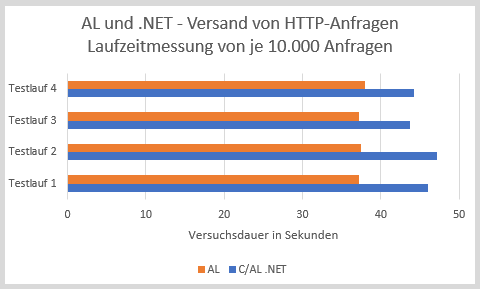
\includegraphics[width=140mm]{images/Tests-WS}
	\caption{Grafische Darstellung der Messergebnisse der Laufzeitmessungen.}
	\label{fig:Test1Graphical}
\end{figure}

Die Messungen zeigen wie erwartet, dass die in die Sprache integrierte Funktionalität ein leicht besseres Laufzeitverhalten zeigt. Trotz des Mehraufwandes des Ladens einer externen Klassenbibliothek und deren Verwendung, verhält sich die AL-Variante jedoch im Durchschnitt lediglich etwa 20\% performanter.
\pagebreak

\section{Tabellenanpassung und Tabellenerweiterung}
Wie im Unterkapitel \textit{Objektarten in Business Central} \ref{fig:TableExtension} erwähnt, können in der erweiterungsbasierten Programmierung unter AL zu bestehenden Tabellenobjekten keine neuen Felder direkt hinzugefügt werden. Um  dennoch die Möglichkeit zu wahren, die Standardtabellen zu erweitern, wurde der Objekttyp der Tabellenerweiterung eingeführt. In Objekten vom Typ Erweiterungstabelle platzierte Felder werden in der Datenbank in einer eigenen Tabelle abgelegt. Diese zusätzliche Tabellen sind unbedingt nötig, um Daten der Erweiterung von denen der Standardapplikation zu kapseln und so zu garantieren, dass die Standardapplikation ohne manuelle Eingriffe mit Updates versorgt werden kann. Gleichzeitig hat dieses Verhalten jedoch auch zur Folge, dass der Zugriff auf die zusätzlichen Felder mit einer \textit{Join-Operation} erfolgen muss. In weiterer Folge können diese Felder auch nicht als \textit{SumIndexField} in einem Tabellenindex verwendet werden kann. 

Ziel der folgenden Testreihe ist es, den Unterschied zwischen einer traditionell zum Tabellenobjekt hinzugefügten Feld, und einem via Erweiterungsobjekt erstellten Feld zu quantifizieren. Zu diesem Zweck wird die C/AL Variante der Tabelle \textit{Loyalty Point Entry} \ref{fig:Tables} mittels einer neuen Erweiterung um ein neues Feld \textit{Points2} erweitert, sodass sich folgendes Tabellenschema ergibt:

\begin{figure}[H]
	\centering
	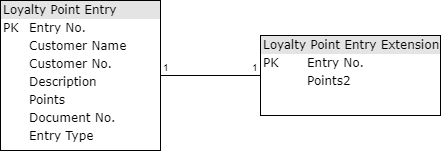
\includegraphics[width=115mm]{images/Test2}
	\caption{Tabellenschema Treuepunktposten und zugehörige Erweiterung.}
	\label{fig:Test2Schema}
\end{figure}

\paragraph{}
Die Abfrage um herauszufinden, wie viele Treuepunkte ein Kunde momentan hat, soll möglichst effizient gestaltet werden. Hierfür wird in der C/AL Variante - also für das Feld \textit{Points} ein nach \textit{Customer No.} gruppierter Index erstellt. Da \textit{Points2} sich auf Datenbankseite nicht in der selben Tabelle befindet, lassen sich derartige Zugriffsoptimierungen via Indizes hier nicht verwirklichen. Für den folgenden Test werden für zehn Kundeneinträge je 10.000 Treuepunktposten erstellt. Gemessen wird die Zeit, welche die Microsoft Dynamics 365 Business Central Instanz benötigt, um für jeden der Kunden den Treuepunktsaldo zu ermitteln. In dieser Messreihe wird das Gesamtsystem bestehend aus Datenbank und  Serverinstanz nach jeder Messung neu gestartet, um Effekte durch Zwischenspeicherungen auszunehmen.

\begin{figure}[H]
	\centering
	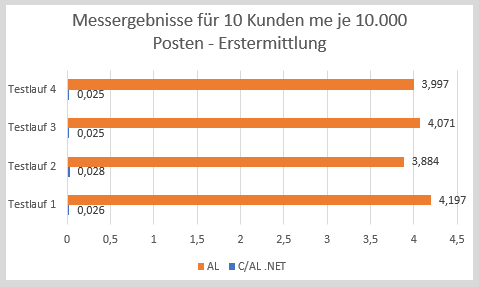
\includegraphics[width=140mm]{images/Test2NoCache}
	\caption{Messung: Aggregierung von Treuepunktposten - Ohne Zwischenspeicher.}
	\label{fig:Test2Schema}
\end{figure}

Hier lässt sich ein deutlicher Unterschied in Bezug auf die Berechnungszeiten feststellen. Die Differenz rührt daher, da das via C/AL erstellte Feld auch gleichzeitig von Microsoft Dynamics 365 Business Central als \textit{SumIndexField} angelegt wurde. Anhand der angegebenen \textit{SumIndexFields} kann Microsoft SQL Server materialisierte Sichten erstellen, um Daten bereits beim Einfügen zu aggregieren. Somit wird beim Zugriff auf das Feld in der C/AL Variante keine Summenoperation ausgeführt, sondern lediglich das Ergebnis aus der materialisierten Sicht wiederverwendet. Währenddessen muss für die Auswertung des Feldes \textit{Points2} aus dem Erweiterungstabellenobjekt jeder Treuepunktposten mit seinem Äquivalent aus der Erweiterungstabelle verbunden werden, und danach die Summe der einzelnen Werte berechnet werden. Dies würde bedeuten, dass jede Berechnung den Nutzer einige Sekunden an Zeit kosten würde. In dieser Testreihe werden lediglich 10.000 Datensätze verwendet, in einem Produktivszenario sind jedoch oft wesentlich größere Datenquellen vorhanden. Um diese Probleme zu mindern, verwendet Microsoft Dynamics 365 Business Central ein komplexes Zwischenspeichersystem, das oft verwendete Datenbestände im Hauptspeicher verwaltet und vor-aggregiert. 
Vor der folgenden Messung wurde das System nicht durchgestartet. Die Serverapplikation hat hier bereits Treuepunktdaten im Hauptspeicher vorberechnet. Dies ist der Zustand in dem sich das System im Normalzustand befindet.
\begin{figure}[H]
	\centering
	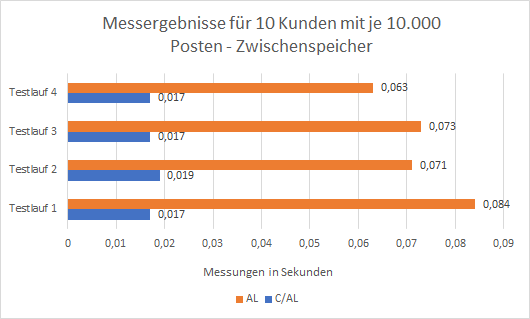
\includegraphics[width=140mm]{images/Test2Cache}
	\caption{Messung: Aggregierung von Treuepunktposten - mit Zwischenspeicher.}
	\label{fig:Test2Schema}
\end{figure}

Der Zugriff und die Berechnung der relevanten Daten dauert in diesem Zustand zwar immer noch etwa vier mal länger, Berechnungszeiten unter 100 Millisekunden sind jedoch bei Operationen dieser Art durchaus vertretbar.

\section{Codeanpassung und ereignisorientierte Codeerweiterung}
Mit der Einführung der Erweiterungsentwicklung und AL, werden den Entwicklern viele neue Möglichkeiten präsentiert. Einerseits ändern sich mit dem erweiterungsbasierten Ansatz Lizenz- und Finanzierungsmodelle, andererseits werden dadurch Entwicklern neue Vertriebsmöglichkeiten zugänglich gemacht. Erweiterungen können ohne Mitwirken des Entwicklers beim Endkunden, und durch den Endkunden selbst installiert werden, da die Integration einer Erweiterung laut technischer Spezifikation keine manuell auszuführenden Tätigkeiten bedingt.

Andererseits werden Entwickler durch diesen Umschwung jedoch auch technologisch eingeschränkt. Anpassungen des Microsoft-Standard Codebestands waren seit Ersterscheinung des ERP-Systems der einzige und bevorzugte Weg, um Änderungen am Verhalten des Systems vorzunehmen. Diese Codeanpassungen geben dem Entwickler vollständige Kontrolle über den Ablauf der einzelnen Teilprozesse im Gesamtsystem. So können Entwickler Programmcode an beliebigen Stellen hinzufügen, bearbeiten oder auch entfernen.

Mit der Einführung der erweiterungsorientierten Entwicklung sind Codeanpassungen nicht mehr möglich. Standard-Applikationsobjekte können nicht mehr verändert werden, lediglich Erweiterungen sind noch möglich. Dies würde jedoch auch bedeuten, dass Entwickler nicht mehr die Möglichkeiten hätten, im Microsoft Standard abgebildete Prozesse abzuändern. Um Entwicklern dennoch Anpassungen der Standardlogik zu ermöglichen, wird seitens Microsoft ein Mechanismus eingeführt, der in anderen Sprachen und Plattformen seit Jahrzehnten zum Standardumfang zählt: Ereignisse (\textit{Events}).

Seit dem Ersterscheinen von Ereignissen in der Version 2016, werden in der gesamtem Applikation und in sämtlichen Prozesslogiken Ereignisse gefeuert. Entwickler können sich an diese Ereignisse binden und je nachdem welche Ereignisse auftreten, spezielle Logikteile ausführen. Mittlerweile befinden sich in der aktuellen Version von Microsoft Dynamics 365 Business Central mehrere tausend Ereignisse, die aus Codeunit-Applikationsobjekten gefeuert werden.

So erlaubt uns ein Ereignis beispielsweise, darauf zu reagieren, nachdem ein Benutzer beim Drucken eines Berichts einen Drucker auswählt. Das Ereignis hierfür kommt aus dem Codeunit-Applikationsobjekt \textit{ReportManagement}, und mit dem folgenden Codestück kann man auf dieses Ereignis reagieren: 

\begin{program}[H]  % Start your code-block
	\begin{JavaCode}
[EventSubscriber(ObjectType::Codeunit, Codeunit::ReportManagement, 'OnAfterGetPrinterName', '', false, false)]
  local procedure OnGetPrinterName(ReportID: Integer; VAR PrinterName: Text[250])
  begin
    //Place custom code here
  end;\end{JavaCode}
\end{program}

Microsoft stellt mit den gefeuerten Ereignissen in der Codebasis tausende Stellen bereit, um sich in die einzelnen Prozessschritte des Gesamtsystems einzuhaken. Zusammenfassend könnte man meinen, dass dadurch die Notwendigkeit von Codeanpassungen vollständig verschwunden wäre. Dem ist jedoch leider nicht so, denn während Ereignisse eine elegante Möglichkeit bieten, Standardvorgehensweisen im System zu manipulieren, hat der Ereignismechanismus auch seine Einschränkungen und Schwächen:

\paragraph{Ausführungsreihenfolge} \mbox{}\\
Was passiert, wenn mehrere Programmstücke auf dasselbe Ereignis reagieren wollen? Konkret geht es darum um die Ausführungsreihenfolge. Welches der reagierenden Codestücke wird zuerst ausgeführt? Da man als Entwickler davon ausgehen muss, dass eine entwickelte Erweiterung auf fremden System ausgeführt wird, ist diese Frage von hoher Wichtigkeit. Denn wenn mehrere Codestücke dieselben Daten ändern, kann es schnell zu Inkonsistenzen kommen. Und inkonsistente Daten können in der Welt der Finanzbuchhaltung schnell zu rechtlichen Schwierigkeiten führen. Bei Änderung eines Systems via Codeanpassung kommt diese Frage nicht auf, die Ausführungsreihenfolge ist strikt durch den Ablauf des Programmcodes gegeben. Auf die Frage, welches Codestück zuerst ausgeführt wird, gibt es keine klare eindeutige Antwort. Im Optimalfall ist der reagierende Code so zu gestalten, dass er weder durch vorhergehende Ereignisbindungen beeinträchtigt wird, noch darauffolgende Ereignisbindungen beeinträchtigt. In sehr vielen Anwendungsfällen ist dies jedoch schlichtweg nicht möglich.

\paragraph{Zugriffseinschränkung} \mbox{}\\
Die Ereignisarchitektur schränkt Entwickler dramatisch ein. Entwickler können nur noch dort eingreifen, wo ein Eingriff seitens Microsoft auch vorgesehen ist. Und selbst an diesen Punkten kann man Prozesse aus der Basisapplikation nur beschränkt modifizieren, da man als Entwickler meist keinen Zugriff auf den Zustand aller lokalen und globalen Variablen innerhalb der aufrufenden Funktion hat. Um das vergleichbares Maß an Flexibilität wie Codeanpassungen zu bieten, wäre praktisch nach jeder Zeile Code in der Standardapplikation eine Ereignisauslösung notwendig.


\section{Source Code Management und CI/CD}
Mit der Nutzung von Visual Studio Code haben Microsoft Dynamics 365 Business Central Entwickler erstmals in der Geschichte der ERP-Lösung Zugriff auf einen modernen dateibasierten Quellcode-Editor \cite{freddysblog}. Programmcode wird nicht mehr primär in einer Entwicklungsdatenbank bearbeitet und gespeichert, sondern befindet sich lokal auf dem Rechner des arbeitenden Entwicklers. Was für Entwickler sämtlicher höherer Programmiersprachen bereits seit Anfang der 90er Jahren Standard ist, gilt seit 2018 auch für Business Central Entwickler. Dabei handelt es sich um einen gigantischen Schritt in die richtige Richtung. 

Im Rahmen der \textit{Mibuso NAVTechDays} \footnote{www.mibuso.com} im November 2018 in Antwerpen, der wohl bedeutendsten Entwicklerkonferenz des Jahres für Dynamics NAV und Business Central Entwickler im europäischen Raum, wurde während eines Vortrags erhoben, wie viele der Anwesenden Entwickler Sourcecode Verwaltungssysteme wie Git für ihre C/AL Projekte verwenden. Die ernüchternde Antwort: nur etwa 10-15\% der anwesenden Entwickler gaben an für C/AL Programmcode ein entsprechendes Verwaltungssystem zu verwenden. Die Gründe hierfür sind naheliegend: Wenn Programmcode nicht bereits während des Entwicklungsprozesses lokal in Dateiform auf dem Entwicklerrechner vorhanden ist, stellt die Nutzung eines Systems wie Git daher einen zusätzlichen Mehraufwand dar, und verkompliziert dadurch den Entwicklungsprozess. Hier ist es oft einfacher und zielführender, nächtlich automatisiert Sicherungen der Entwicklungsdatenbank beziehungsweise aller Applikationsobjekte zu erstellen, und diese bei Bedarf wiederherzustellen.

Mit AL und Visual Studio Code sind diese Einschränkungen Vergangenheit. Als Entwickler für Microsoft Dynamics 365 Business Central hat man nun Zugang zu einer modernen Entwicklungsumgebung mit vollständiger Integration in die Quellcode-Verwaltungssoftware Git. 

\paragraph{}
Mit all diesen Neuerungen werden nun auch die Themen \textit{Continuous Integration} und \textit{Continuous Deployment} - kurz \textit{CI/CD} für Business Central Entwickler immer interessanter. Bei \textit{Continuous Integration} handelt es sich um ein Vorgehen in der Softwareentwicklung, bei dem Mitarbeiter an einem Softwareprojekt die von ihm getätigten Änderungen mehrmals täglich in den Hauptentwicklungsstrang integriert \cite{fowler2006continuous}. Die durchgeführten Änderungen werden im Laufe dieser Integration sofort kompiliert und anhand verschiedener Kriterien getestet. Das wichtigste Testkriterium sind hier durch die Entwickler erstellten Testfälle. Sollte ein Testfall fehlschlagen, so wird die getätigte Änderung verworfen, und der verantwortliche Mitarbeiter darüber informiert. So kann schnellstmöglich auf Fehler reagiert werden. 
 
Die Aufgabe des \textit{Continuous Deployment} besteht darin, erfolgreich integrierte Änderungen auch direkt in Anwendungsform verfügbar zu machen. Im Business Central Umfeld bedeutet das typischerweise, automatisiert ein Online-Testsystem zu erstellen, das mit der aktuellen Version der entwickelten Erweiterung bestückt wird und so für Entwickler, Tester und auch den Endkunden zugänglich ist. Das erstellte Testsystem arbeitet vorzugsweise auf einer Kopie der Kundendatenbank, um möglichst realitätsnahe Verhältnisse zu schaffen.

Diese beiden Entwicklungsmodelle abzubilden ist mit dem Development Environment und AL schier unmöglich. Einerseits gibt es keine Möglichkeit, Applikationsobjekte ohne der Nutzung des Development Environment zu kompilieren. Andererseits ist auch die Integration von bereits erstellten Applikationsobjekten im Binär- oder Textformat komplex und dadurch fehleranfällig. Da ein großer Teil der Entwickler C/AL Applikationen ohnehin auf zentralen Entwicklungsdatenbanken und ohne Quellcodeverwaltung entwickeln, stellt sich die Frage der Notwendigkeit eines \textit{CI/CD} Systems oft erst gar nicht. 

In der cloudbasierten Zukunft von Microsoft Dynamics 365 Business Central bringt der Einsatz derartiger \textit{CI/CD} Systeme einige Vorteile. So können einzelnen Kunden ohne Mehraufwand aktuelle Testsysteme zur Verfügung gestellt werden, anhand deren neue Funktionalitäten präsentiert und getestet werden können. Aufgaben wie die Erstellung eines neuen Testsystems anhand der aktuellsten Versionen des Grundsystems mit der Eigenentwicklung, basierend auf Kundendaten können in der C/AL Welt durchaus mehrere Stunden in Anspruch nehmen. Mit einem cloudbasierten System und einem geeignetem \textit{CI/CD} Prozess kann diese Aufgabe automatisiert, vorhersehbar und zeitnah innerhalb weniger Minuten ausgeführt werden. Leider gibt es seitens Microsoft bezüglich \textit{CI/CD} noch keine offiziellen Empfehlungen oder bewährte Verfahren. So sind Entwickler in diesem Aspekt leider noch vollkommen auf sich selbst angewiesen. Es ist jedoch davon auszugehen, dass Microsoft hier in Zukunft entsprechende Konfigurationen zur Verfügung stellen wird. 




